\section{Results}
\label{sec:results}

In this section, we present our findings based on the implementation of the efficient UQ computational framework 
presented in Section~\ref{sec:method}, based on identifying an active subspace that captures the variability
in bulk thermal conductivity of Si due to uncertainty in the SW potential parameters. As discussed earlier, the
active subspace helps transform the dependence of the model output $G$ on a large set of uncertain physical
inputs into an equivalent low-dimensional function $\mathcal{Y}$ in the active subspace. 
Thus $\mathcal{Y}$ depends on a much smaller set of independent variables $\vec\eta$,
referred to as active variables. While dimension reduction due to active subspace
 increases computational efficiency, the computation of the subspace itself is further enhanced in efficiency
by means of a regression fit to the trend exhibited by $\mathcal{Y}(\vec{\eta})$. Since the active subspace is
observed to be 1-dimensional in the present case, a simple linear regression fit is adequate for constructing
a surrogate model, $\tilde{\mathcal{Y}}(\vec{\eta})$.
The accuracy of the surrogate was assessed by first evaluating the 
relative L$^2$ norm of the discrepancy between NEMD-based estimates and surrogate predictions,
and second, by comparing probability distributions of the bulk thermal conductivity obtained using
model evaluations and the surrogate. The surrogate was exploited to perform a GSA of the SW
potential parameters as well as for evaluating a joint likelihood of the important parameters.

\subsection{Computing the Active Subspace}
\label{sub:cas}

The iterative procedure outlined in Algorithm~\ref{alg:free} was used to compute the active subspace. 
We began
with an initial set of 5 samples in the 7-dimensional input space. The Monte Carlo samples were drawn
from the joint prior distribution of the uncertain SW parameters, assumed
to be uniformly distributed in the interval $[0.9\theta_i^\ast,1.1\theta_i^\ast]$, where $\theta_i^\ast$ are the
nominal values provided in Table~\ref{tab:sw}. 
%
\begin{table}[htbp]
\centering
\ra{1.3}
\begin{tabular}{@{}ccccccc@{}}\toprule
$A$ & $B$ & $p$ & $q$ & $\alpha$ & $\lambda$ & $\gamma$ \\
7.05 & 0.60 & 4.0 & 0.0 & 1.80 & 21.0 & 1.20 \\
\bottomrule
\end{tabular}
\caption{Nominal values of the SW potential parameters~\cite{Stillinger:1985}.}
\label{tab:sw}
\end{table}
%
An initial set of model evaluations was used to estimate the gradient vector of thermal conductivity w.r.t.
individual components representing the derivative with respect to $\xi_i$ corresponding to $\theta_i$ in
the physical space. At each iteration, $i$, model evaluations at 5 new samples in the full space were 
obtained and the quantity, $\vec{\varepsilon}^{(i)}$ was computed using~\eqref{eq:conv}. The iterative
procedure was terminated once the highest component of $\vec{\varepsilon}^{(i)}$ was found to be smaller than
the specified tolerance, $\tau$ = 0.1. In this case, the process was observed to converge after 4 iterations,
and required model evaluations at 25 samples, yielding $\max(\vec{\varepsilon}^{(i)})$~=~0.085.
 The resulting active subspace was found to be
1-dimensional. In Figure~\ref{fig:casfig1}, we plot the components of the dominant eigenvector (left),
and the quantity, $\max(\vec{\varepsilon}^{(i)})$, computed using components of the dominant eigenvector 
obtained between successive iterations, $i$ and $i-1$ (right) in~\eqref{eq:conv}.
%
\begin{figure}[htbp]
\begin{center}
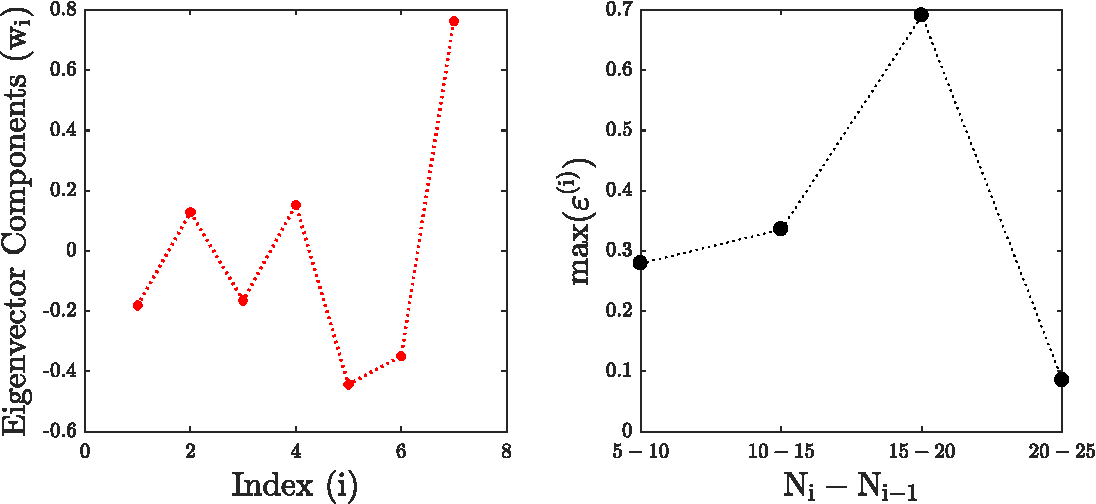
\includegraphics[width=0.8\textwidth]{./Figures/free_eigv5}
\caption{Left: Individual components of the dominant eigenvector that constitute the 1-dimensional
active subspace. Right: A plot of $\max(\varepsilon^{(i)})$, obtained
using components of the dominant eigenvector between successive iterations.}
\label{fig:casfig1}
\end{center}
\end{figure}
%

The normalized eigenvalue spectrum is illustrated
in Figure~\ref{fig:casfig2}~(left), and the plot of $\mathcal{Y}$ vs. $\vec\eta$, regarded as the \textit{sufficient
summary plot} (SSP) is provided in Figure~\ref{fig:casfig2}~(right). Note that the surrogate $\tilde{\mathcal{Y}}$
represented by the straight-line is also illustrated.
%
\begin{figure}[htbp]
\begin{center}
\begin{tabular}{cc}
  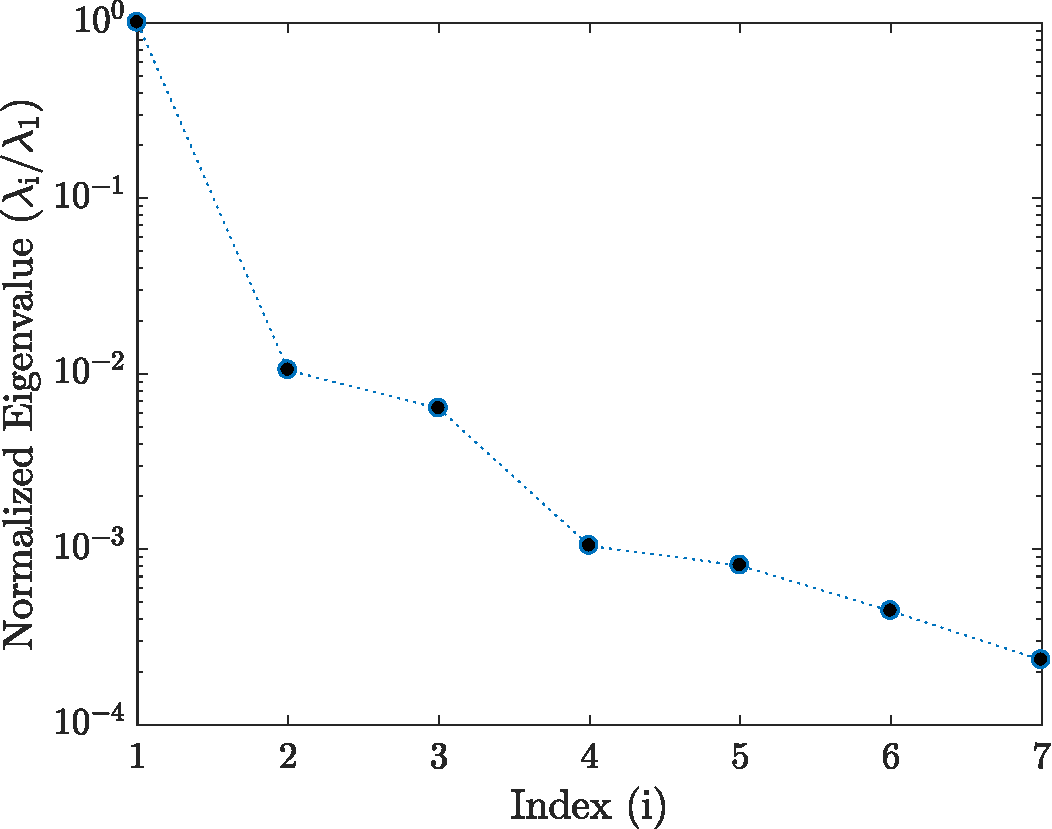
\includegraphics[width=0.42\textwidth]{./Figures/eig_spec}
  &
  \hspace{3mm}
  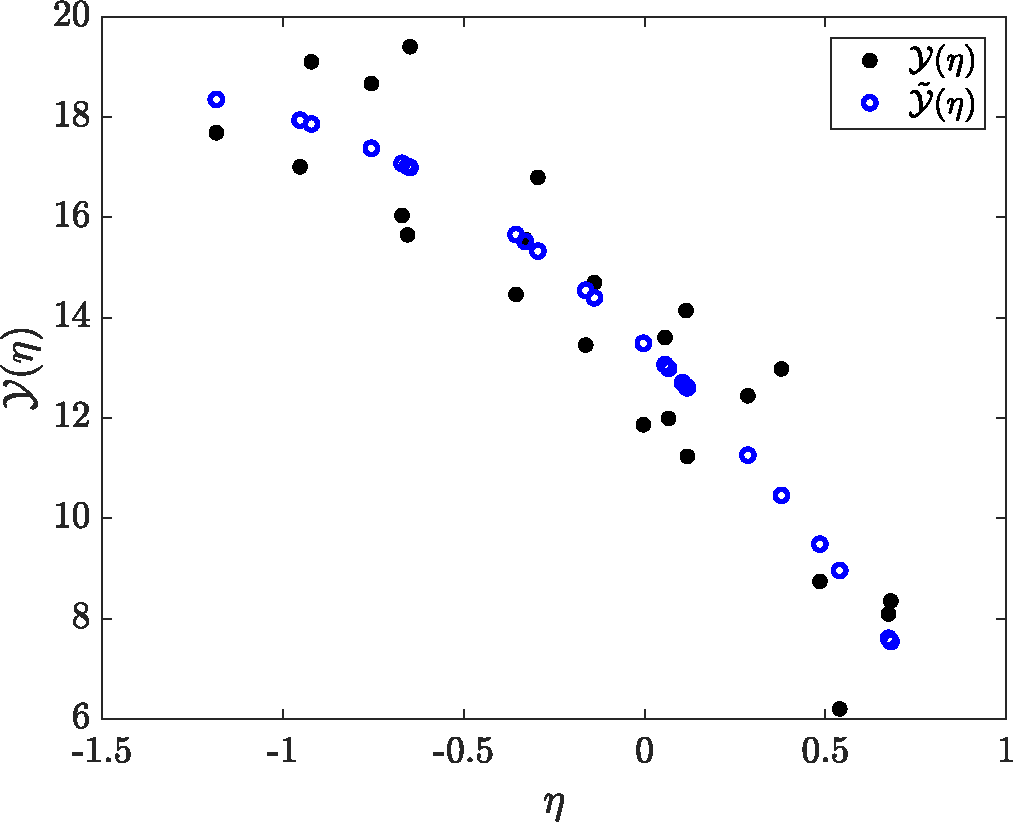
\includegraphics[width=0.4\textwidth]{./Figures/free_ssp1D}
  \end{tabular}
\caption{Left: Normalized eigenvalue spectrum of the converged matrix, $\hat{\mat{C}}$. Right: SSP
illustrating the variability of the NEMD-based thermal conductivity estimates in the 1-dimensional
active subspace.}
\label{fig:casfig2}
\end{center}
\end{figure}
%
The normalized eigenvalue spectrum
shows that the ratio of the first two eigenvalues, $\left(\frac{\lambda_1}{\lambda_2}\right)\sim\mathcal{O}(10^2)$.
Thus, the second largest eigenvalue is roughly two orders of magnitude smaller than the largest eigenvalue,
indicating a 1-dimensional active subspace. Furthermore, the trends in the SSP seem to have been captured
reasonably well using a linear regression fit which further confirms the existence of a 1-dimensional active
subspace in this case. In the following section, we verify the accuracy of the
surrogate $\tilde{\mathcal{Y}}$. 


\subsection{Surrogate assessment}
\label{sub:ver}

The surrogate $\tilde{\mathcal{Y}}$ illustrated in Figure~\ref{fig:casfig2}~(right) 
is assessed for accuracy at two levels: First, we estimate
 the relative L$^2$ norm of the difference
($\varepsilon_d$) between surrogate predictions and NEMD-based estimates of bulk thermal conductivity 
of the Si bar ($\mathcal{Y}$) as follows:
%
\be
\varepsilon_d = \frac{\|\mathcal{Y}(\bm{\eta}) - \tilde{\mathcal{Y}}(\bm{\eta})\|_2}{\|\mathcal{Y}(\bm{\eta})\|_2}
\ee
%
The quantity $\varepsilon_d$ was estimated to be roughly 0.1. In other words, the error introduced
due to approximating the function $\mathcal{Y}$ by a surrogate $\tilde{\mathcal{Y}}$ is about 10$\%$.
For many applications, this error might be too large; however, it is reasonable and
potentially acceptable for this problem considering that we are interested in approximating
the variability in thermal conductivity due to uncertainty in the SW
parameters. Uncertainty propagation analysis using a 7-dimensional input space for an application involving
atomistic simulations would be computationally impractical as discussed earlier in
Section~\ref{sec:intro}, and highlighted specifically in Table~\ref{tab:effort}.

A second assessment of $\tilde{\mathcal{Y}}$ is performed wherein
the first-order and second-order 
statistics as well as probability distributions, obtained using the
surrogate and the set of available model evaluations at 35 samples in the 7-dimensional
input space are compared. Table~\ref{tab:verify} provides estimates of the
mean and the standard deviation of bulk thermal conductivity based on the model and the
surrogate. 
%
\begin{table}[htbp]
\begin{center}
\begin{tabular}{ccc}
\toprule
$\textbf{Distribution}$ & $\mu$ & $\sigma$ \\ 
\bottomrule
$G$~(Model) & 13.764 & 3.573 \\
$\tilde{\mathcal{Y}}$ (1D Surrogate) & 13.757 & 3.441 \\
\bottomrule
\end{tabular}
\end{center}
\caption{Mean ($\mu$) and standard deviation ($\sigma$) corresponding to
the model evaluations ($G$) and surrogate predictions ($\tilde{\mathcal{Y}}$)
at 35 samples in the cross-validation set.}
\label{tab:verify}
\end{table}
%
Figure~\ref{fig:level2} illustrates a comparison of a histogram based on the 35 model evaluations
and a probability density function (PDF), generated using kernel density estimation (KDE)
of surrogate predictions at 10$^5$ Monte Carlo samples in the 7-dimensional input domain. 
\begin{figure}[htbp]
\begin{center}
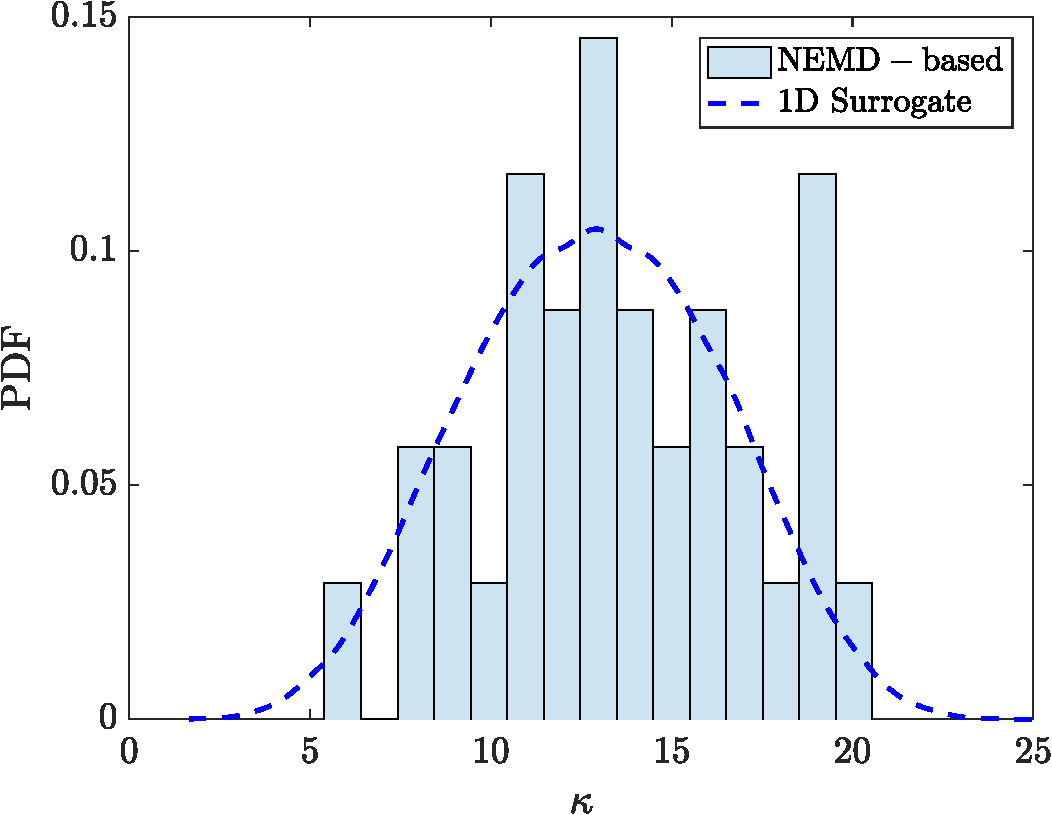
\includegraphics[width=3.0in]{./Figures/free_pdf_comp_SSP1D}
\end{center} 
\caption{A illustrative comparison of the histogram plot based on the
available set of 35 model evaluations and a PDF generated using surrogate predictions at 10$^5$
random samples in the 7-dimensional input domain.}  
\label{fig:level2}
\end{figure}
%
From the values reported in Table~\ref{tab:verify}, it can be said that the
 first-order ($\mu$) and second-order ($\sigma$) statistics of the bulk thermal conductivity ($\kappa$),
obtained using the model and the surrogate  are found to be in close agreement. Additionally, the
comparison of distributions in Figure~\ref{fig:level2} confirms that the PDF captures the modal
estimate as well as the spread in $\kappa$ with reasonable accuracy. Hence, the surrogate based on
the 1-dimensional active subspace, evaluated earlier in~\ref{sub:cas} can be used to quantify and
characterize the uncertainty in bulk thermal conductivity of the Si bar due to the uncertainty in the
SW potential parameters. In the following section, we use the surrogate to estimate the 
total effect Sobol'
sensitivity indices of the SW parameters. Additionally, we perform a consistency check by comparing
these estimates with the normalized activity scores, computed using the converged 1-dimensional
active subspace. 

\subsection{Global Sensitivity Analysis}
\label{sub:gsa}

The surrogate $\tilde{\mathcal{Y}}(\vec{\eta})$ was used to estimate the total effect Sobol'
 index, $T_i(G)$ for each
uncertain parameter by mapping 10$^5$ independent Monte Carlo samples in the physical domain
to the bulk thermal conductivity of the Si bar as discussed earlier in~\ref{subsub:gsa_surr}. 
Additionally, normalized activity scores ($\nu_{i,p}$) were computed using~\eqref{eq:ac} and~\eqref{eq:nac}.
A bar-graph comparing estimates of $T_i(G)$ and $\nu_{i,p}$ is provided in
Figure~\ref{fig:gsa}. 
%
\begin{figure}[htbp]
\begin{center}
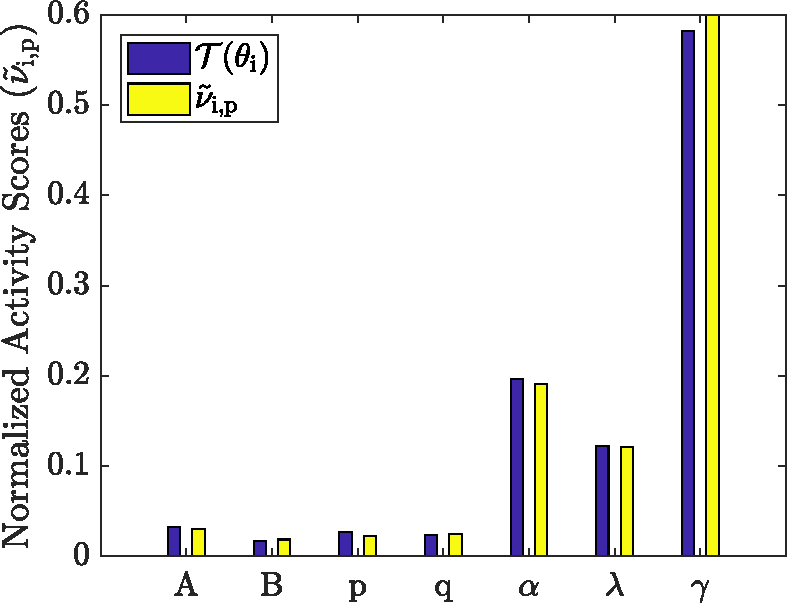
\includegraphics[width=0.45\textwidth]{./Figures/free_as_gsa}
\caption{A comparative assessment of the total effect Sobol' index, $T_i(G)$, and the normalized
activity scores, $\tilde{\nu}_{i,p}$, for GSA of the SW potential parameters.}
\label{fig:gsa}
\end{center}
\end{figure}
%
The sensitivity trends from the two approaches are found to be consistent. This is expected since
both, the surrogate and the dominant eigenvectors are associated with the same 1-dimensional active 
subspace. However, the quantitative agreement in the estimates of $T_i(G)$ and $\tilde{\nu}_{i,p}$
is purely coincidental. The trends observed in Figure~\ref{fig:gsa} indicate
 that the variability in bulk thermal conductivity is predominantly
due to the uncertainty in $\alpha$, $\lambda$, and $\gamma$. This is also consistent with our earlier
findings based on the derivative-based global sensitivity measures~\cite{Vohra:2018b}~(see Figure~7 therein). 
This result could be exploited for the purpose of optimal allocation of computing resources to calibrate
the key contributors ($\alpha$, $\lambda$, and $\gamma$) to the variability in the bulk thermal conductivity
predictions from NEMD simulations of the Si bar. 

In the following section, we use the active subspace-based surrogate model
for calibrating the important SW parameters in a Bayesian
setting as discussed earlier in~\ref{sub:ba_method}.
 For the purpose of illustration, we focus on estimating posterior distributions of
 the two main contributors to the QoI variability, i.e.,
$\alpha$ and $\gamma$. 

\subsection{Bayesian calibration}
\label{sub:ba}

Herein, the parameters for calibration, $\alpha$ and $\gamma$ are considered to be independent and
uniformly distributed in the intervals, [1.62, 1.98] and [1.08, 1.32] respectively. The joint posterior,
$\mathbb{P}(\bm{\theta}\vert \bm{D})$ in ~\eqref{eq:bayes} is thus 
proportional to the joint likelihood, modeled using a Gaussian distribution:
%
\be
\mathbb{P}(\bm{D}\vert\bm{\theta}) = \frac{1}{\sqrt{2\pi\sigma^2}}\exp\left[-\frac{(\kappa_{\tiny{\mbox{E}}} - 
\kappa_{\tiny{\mbox{MD}}})^2}{2\sigma^2}\right],
\label{eq:like}
\ee
%
\noindent where $\sigma$ is the standard deviation associated with measurement error, and
$(\kappa_{\tiny{\mbox{E}}} - \kappa_{\tiny{\mbox{MD}}})$ is the discrepancy between 
NEMD predictions~($\kappa_{\tiny{\mbox{MD}}}$) and measurements~($\kappa_{\tiny{\mbox{E}}}$). 
Note that repeated evaluations of the joint likelihood can be remarkably challenging since it involves 
$\kappa_{\tiny{\mbox{MD}}}$. As mentioned earlier in~\ref{sub:ba_method}, we overcome this challenge by
exploiting the surrogate
$\tilde{\mathcal{Y}}(\vec{\eta})$ to map samples in the physical space to the estimates of 
$\kappa_{\tiny{\mbox{MD}}}$, in~\eqref{eq:like}.

The joint likelihood was evaluated on a 2D cartesian grid containing 40$\times$40 samples, and is shown
using a contour plot in Figure~\ref{fig:like}(a). Note that 
$\kappa_{\tiny{\mbox{E}}}$~=~149~W/m/K~\cite{Shanks:1963} at 300~K, and a $\sigma$ value, 
0.15$\ast$$\kappa_{\tiny{\mbox{E}}}$, was used to evaluate the joint likelihood.
Marginal likelihoods for  $\alpha$ and $\gamma$ are also
shown in Figures,~\ref{fig:like}(b) and~\ref{fig:like}(c) respectively. 
%
\begin{figure}[htbp]
 \begin{center}
  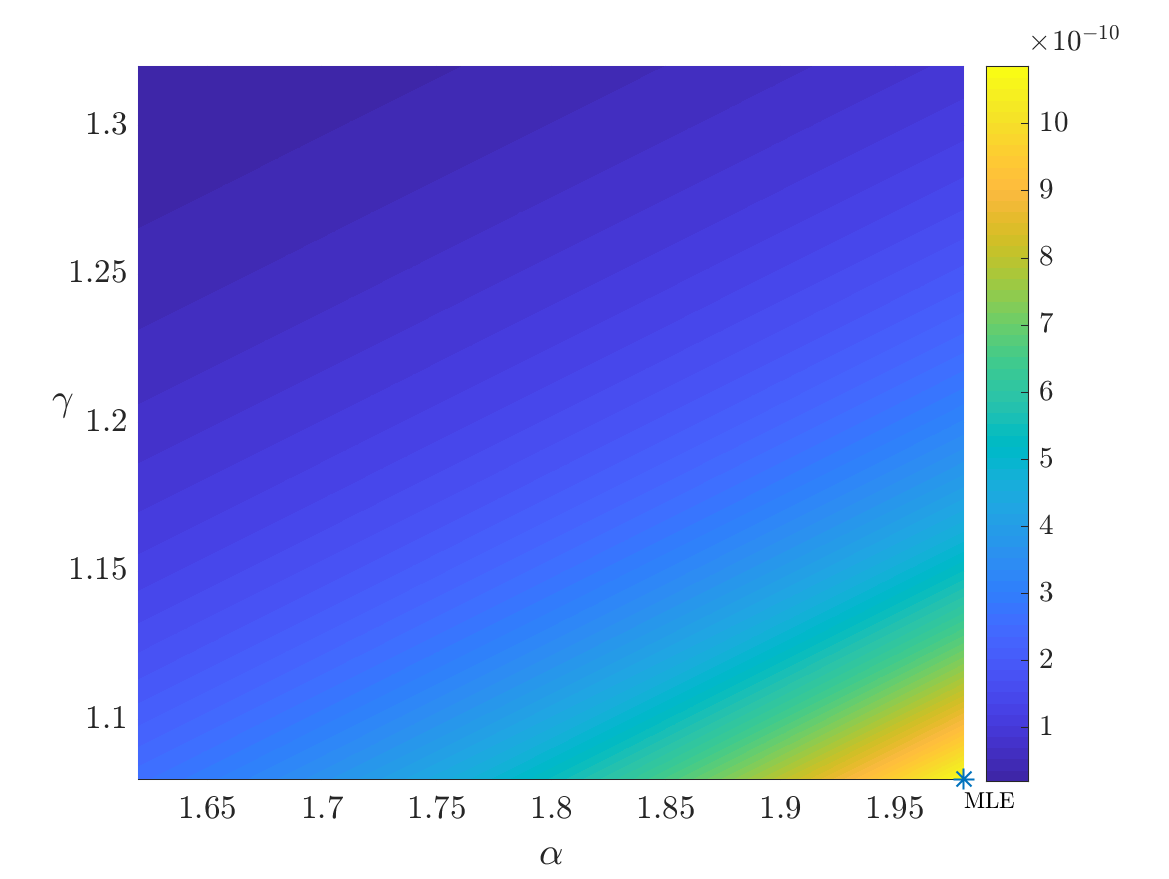
\includegraphics[width=0.50\textwidth]{./Figures/gl}
  \\ (a) \\
  \begin{tabular}{cc}
  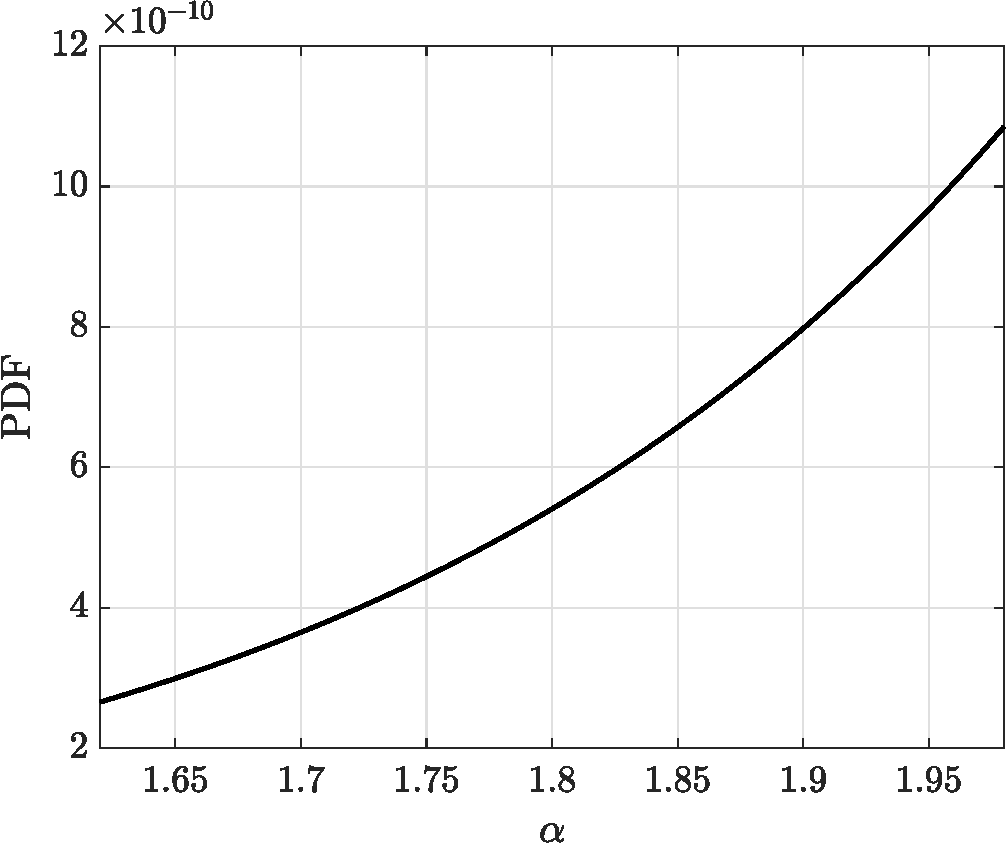
\includegraphics[width=0.37\textwidth]{./Figures/pdf_alpha}
  &
  %\hspace{3mm}
  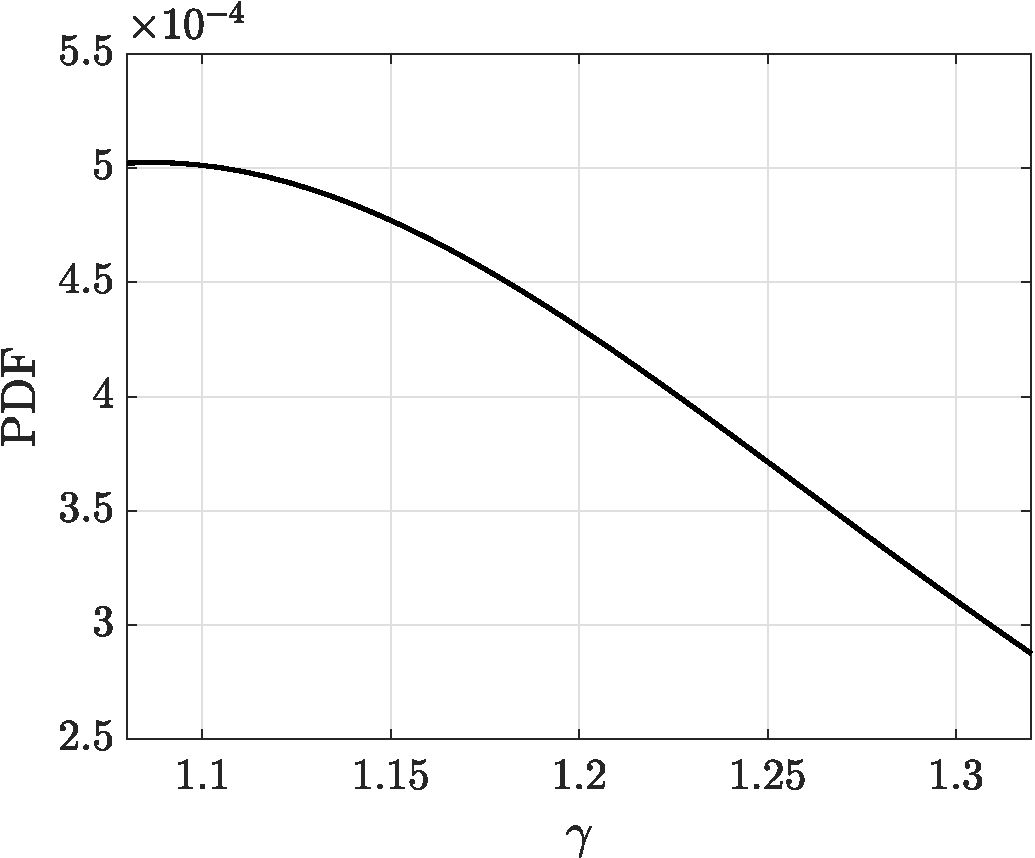
\includegraphics[width=0.37\textwidth]{./Figures/pdf_gamma}
  \\ (b) & (c)
  \end{tabular}
\caption{(a) The joint likelihood of ($\alpha$,$\gamma$), estimated using Eq.~\ref{eq:like} is plotted
on a (40$\times$40) 2D cartesian grid. The maximum likelihood estimate (MLE) is also highlighted.
Marginal likelihoods for $\alpha$ and $\gamma$ are shown in (b) and (c) respectively.}
\label{fig:like}
\end{center}
\end{figure}
%
Note that the joint likelihood was evaluated using a single data point for 
$\kappa_{\tiny{\mbox{E}}}$ at 300~K. An enriched set of data would help improve the accuracy
of the calibration process, and thus refine the posterior distributions of $\alpha$ and $\gamma$.
However, an active subspace will need to be identified for each temperature at which the data is 
available, thus requiring a significant amount of computational effort, and is not pursued here. 
However, it must be noted that since the computational
effort at each temperature is significantly reduced by dimension reduction as shown here,
the overall effort is still expected to be several orders of magnitude smaller than 
that required when using atomistic simulations for calibrating all the SW parameters.
It is encouraging to note that the joint likelihood obtained using the active subspace methodology
in this work exhibits qualitative as well as quantitative agreement with that computed using
the same data point, and a reduced-space polynomial chaos surrogate with a 5-dimensional
Legendre polynomial basis in~\cite{Vohra:2018a} (see Figure~11 therein). 






























